% !TeX program = xelatex
\documentclass[a4paper,10pt]{article}

% ============================================================================
% ១. កញ្ចប់បណ្ណាល័យ និងការកំណត់ទំព័រ (Packages & Page Setup — តាមគំរូ ls_plan.tex)
% ============================================================================
\usepackage[a4paper, left=0.95cm, right=0.95cm, top=0.85cm, bottom=0.92cm, footskip=0.52cm]{geometry}
\usepackage{amsmath}
\usepackage{unicode-math}
\usepackage{fontspec}
\usepackage{longtable, array, multirow, colortbl}
\usepackage[table]{xcolor}
\usepackage{enumitem}
\usepackage{pifont}
\usepackage{fancyhdr}
\usepackage{tikz}
\usetikzlibrary{calc, arrows.meta, decorations.pathreplacing, patterns, positioning, babel}

\makeatletter
\let\@expl@@@mark@update@singlecol@structures@@\relax
\makeatother

% --- ប្រព័ន្ធស្វែងរកទីតាំងពុម្ពអក្សរស្វ័យប្រវត្តិ (Windows Local + Cloud Repo fonts/) ---
\providecommand{\NGSFindFonts}{%
  \IfFileExists{C:/Windows/Fonts/cambria.ttc}{%
    \def\NGSSysPath{C:/Windows/Fonts/}%
    \def\NGSUserPath{C:/Users/KIT/AppData/Local/Microsoft/Windows/Fonts/}%
  }{%
    \IfFileExists{./fonts/KhmerOSsiemreap.ttf}{\def\NGSSysPath{./fonts/}\def\NGSUserPath{./fonts/}}{%
    \IfFileExists{../fonts/KhmerOSsiemreap.ttf}{\def\NGSSysPath{../fonts/}\def\NGSUserPath{../fonts/}}{%
    \IfFileExists{../../fonts/KhmerOSsiemreap.ttf}{\def\NGSSysPath{../../fonts/}\def\NGSUserPath{../../fonts/}}{%
    \IfFileExists{../../../fonts/KhmerOSsiemreap.ttf}{\def\NGSSysPath{../../../fonts/}\def\NGSUserPath{../../../fonts/}}{%
    \IfFileExists{../../../../fonts/KhmerOSsiemreap.ttf}{\def\NGSSysPath{../../../../fonts/}\def\NGSUserPath{../../../../fonts/}}{%
    \IfFileExists{../../../../../fonts/KhmerOSsiemreap.ttf}{\def\NGSSysPath{../../../../../fonts/}\def\NGSUserPath{../../../../../fonts/}}{%
    \IfFileExists{../../../../../../fonts/KhmerOSsiemreap.ttf}{\def\NGSSysPath{../../../../../../fonts/}\def\NGSUserPath{../../../../../../fonts/}}{%
      \def\NGSSysPath{../../../../../../../fonts/}\def\NGSUserPath{../../../../../../../fonts/}%
    }}}}}}}%
  }%
}
\NGSFindFonts

% ============================================================================
% ២. កំណត់ពុម្ពអក្សរ (Fonts — តាមគំរូ ls_plan.tex)
% ============================================================================
\setmathfont[Path={\NGSSysPath}, FontIndex=1, Scale=1.02]{cambria.ttc}
\defaultfontfeatures{Ligatures=TeX}

\setmainfont[
  Path={\NGSUserPath},
  Extension=.ttf,
  Script=Khmer,
  BoldFont={KhmerOSsiemreap},
  BoldFeatures={FakeBold=1.8},
  ItalicFont={KhmerOSsiemreap},
  ItalicFeatures={FakeSlant=0.25},
  BoldItalicFont={KhmerOSsiemreap},
  BoldItalicFeatures={FakeBold=1.8, FakeSlant=0.25}
]{KhmerOSsiemreap}

\newfontfamily\muol[Path={\NGSUserPath}, Extension=.ttf, Script=Khmer]{KhmerOSmuollight}
\newfontfamily\Tacteing[Path={\NGSUserPath}, Extension=.TTF]{TACTENG}
\newfontfamily\TimesEn[Path={\NGSSysPath}, Extension=.ttf, BoldFont={timesbd}, ItalicFont={timesi}, BoldItalicFont={timesbi}]{times}
\newfontfamily\CalibriFont[Path={\NGSSysPath}, Extension=.ttf]{calibri}
\newfontfamily\CourierCirc[Path={\NGSSysPath}, Extension=.ttf]{cour}

\XeTeXlinebreaklocale "km"
\XeTeXlinebreakskip = 0pt plus 1pt minus 0.1pt

% ============================================================================
% ៣. ពណ៌ និងការតុបតែង (Colors & Styles)
% ============================================================================
\definecolor{stepbg}{HTML}{D9D9D9}
\definecolor{headgray}{HTML}{E6E6E6}
\definecolor{emphred}{HTML}{C00000}

\pagestyle{fancy}
\fancyhf{}
\renewcommand{\headrulewidth}{0pt}
\fancyfoot[R]{\CalibriFont\fontsize{9pt}{11pt}\selectfont\thepage}

\setlength{\parindent}{0pt}
\setlength{\parskip}{0pt}
\setlength{\tabcolsep}{4.5pt}
\setlength{\LTpre}{2pt}
\setlength{\LTpost}{2pt}

\newcolumntype{L}[1]{>{\raggedright\arraybackslash}p{#1}}
\newcolumntype{C}[1]{>{\centering\arraybackslash}p{#1}}

% ============================================================================
% ៤. ពាក្យបញ្ជាជំនួយ (Helper Macros)
% ============================================================================
\newcommand{\en}[1]{{\TimesEn #1}}
\newcommand{\enbf}[1]{{\TimesEn\bfseries #1}}
\newcommand{\khmflourish}{{\Tacteing\fontsize{15pt}{15pt}\selectfont 3}}
\newcommand{\wcirc}{{\CourierCirc\fontsize{9.5pt}{11pt}\selectfont o}}
\newcommand{\ditem}{{\fontsize{7.5pt}{10pt}\selectfont\ding{117}}\ }
\newcommand{\fiveE}[1]{\textcolor{emphred}{\CalibriFont\bfseries #1}}
\newcommand{\redsub}[1]{\textcolor{emphred}{#1}}
\newcommand{\timenote}[1]{\textcolor{emphred}{\textit{#1}}}
\newcommand{\stepheader}[1]{\multicolumn{3}{|c|}{\cellcolor{stepbg}\muol #1} \\ \hline}
\newcommand{\cfig}[1]{{\centering\vspace{3pt}#1\vspace{3pt}\par}}
\newcommand{\cnum}[1]{\mbox{\fontsize{10.5pt}{12pt}\selectfont\ding{\numexpr181+#1\relax}}}
\newcommand{\unit}[1]{\,\text{\en{#1}}}
\newcommand{\graybox}[1]{\colorbox{headgray}{\strut #1}}

% ============================================================================
% ៥. រូបភាព TikZ ស-ខ្មៅ សម្រាប់បង្រៀនលើក្ដារខៀន និងសន្លឹកកិច្ចការ (B&W Diagrams)
% ============================================================================

% ១. E1 Engage: អន្ទាក់ការគណនាការេ 5^2 និងគូប 5^3 (៨.១ ទំ.១២)
\newcommand{\figEngageWNOneSeven}{%
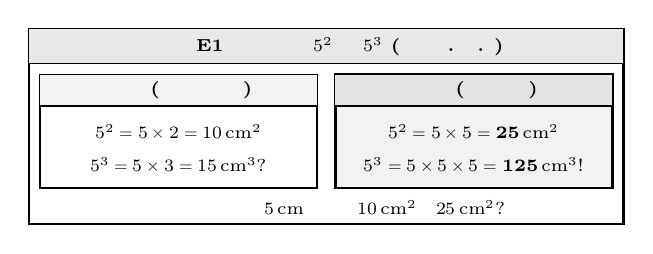
\begin{tikzpicture}[x=1cm, y=1cm, every node/.style={font=\fontsize{6.3pt}{8.3pt}\selectfont, text=black}]
  \draw[black, line width=0.9pt] (0,0) rectangle (7.55,2.48);
  \fill[gray!18] (0,2.04) rectangle (7.55,2.48);
  \draw[black, line width=0.6pt] (0,2.04) -- (7.55,2.04);
  \node at (3.775,2.26) {\textbf{បេសកកម្ម \en{E1}៖ អន្ទាក់ការគណនា $5^2$ និង $5^3$ (ឧទាហរណ៍ ៨.១ ទំ.១២)}};

  % Left: Student A
  \draw[black, line width=0.8pt] (0.14,0.46) rectangle (3.66,1.90);
  \fill[gray!10] (0.14,1.50) rectangle (3.66,1.90);
  \draw[black, line width=0.5pt] (0.14,1.50) -- (3.66,1.50);
  \node at (1.90,1.70) {\textbf{សិស្ស ក (ច្រឡំគុណនិទស្សន្ត)}};
  \node at (1.90,1.18) {$5^2 = 5 \times 2 = 10\unit{cm}^2$};
  \node at (1.90,0.76) {$5^3 = 5 \times 3 = 15\unit{cm}^3$?};

  % Right: Student B
  \draw[black, line width=0.95pt, fill=gray!10] (3.89,0.46) rectangle (7.41,1.90);
  \fill[gray!22] (3.89,1.50) rectangle (7.41,1.90);
  \draw[black, line width=0.55pt] (3.89,1.50) -- (7.41,1.50);
  \node at (5.65,1.70) {\textbf{សិស្ស ខ (គុណកត្តាដដែលៗ)}};
  \node at (5.65,1.18) {$5^2 = 5 \times 5 = \mathbf{25}\unit{cm}^2$};
  \node at (5.65,0.76) {$5^3 = 5 \times 5 \times 5 = \mathbf{125}\unit{cm}^3$!};

  \node at (3.775,0.21) {\textbf{សំណួរ៖} តើផ្ទៃការេជ្រុង $5\unit{cm}$ មានក្រឡា $10\unit{cm}^2$ ឬ $25\unit{cm}^2$?};
\end{tikzpicture}}

% ២. E2 Explore: រូបធរណីមាត្រការេ-គូប និងឫសការេ-ឫសគូប (៨.១ និង ៨.២ ទំ.១២)
\newcommand{\figGeomWNOneSeven}{%
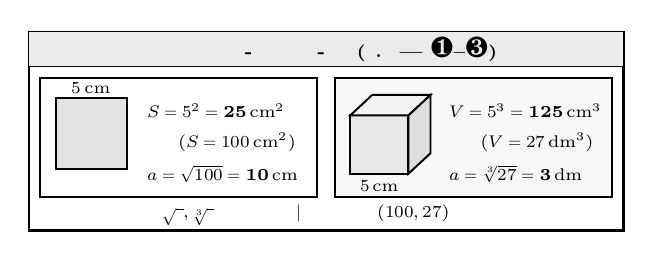
\begin{tikzpicture}[x=1cm, y=1cm, every node/.style={font=\fontsize{6.1pt}{8.0pt}\selectfont, text=black}]
  \draw[black, line width=0.9pt] (0,0) rectangle (7.55,2.52);
  \fill[gray!16] (0,2.08) rectangle (7.55,2.52);
  \draw[black, line width=0.6pt] (0,2.08) -- (7.55,2.08);
  \node at (3.775,2.30) {\textbf{គំរូធរណីមាត្រនៃការេ-គូប និងឫសការេ-ឫសគូប (ទំ.១២ — \cnum{1}--\cnum{3})}};

  % Left: Square 5cm & S=100
  \draw[black, line width=0.8pt] (0.14,0.42) rectangle (3.66,1.94);
  \fill[gray!22] (0.34,0.78) rectangle (1.24,1.68);
  \draw[black, line width=0.75pt] (0.34,0.78) rectangle (1.24,1.68);
  \node at (0.79,1.81) {$5\unit{cm}$};
  \node[anchor=west] at (1.38,1.52) {$S = 5^2 = \mathbf{25}\unit{cm}^2$};
  \node[anchor=west] at (1.38,1.12) {ច្រាស ($S=100\unit{cm}^2$)៖};
  \node[anchor=west] at (1.38,0.72) {$a = \sqrt{100} = \mathbf{10}\unit{cm}$};

  % Right: Cube 5cm & V=27
  \draw[black, line width=0.8pt, fill=gray!6] (3.89,0.42) rectangle (7.41,1.94);
  \draw[black, line width=0.75pt, fill=gray!18] (4.08,0.72) rectangle (4.82,1.46);
  \draw[black, line width=0.7pt, fill=gray!10] (4.08,1.46) -- (4.36,1.72) -- (5.10,1.72) -- (4.82,1.46) -- cycle;
  \draw[black, line width=0.7pt, fill=gray!26] (4.82,0.72) -- (5.10,0.98) -- (5.10,1.72) -- (4.82,1.46) -- cycle;
  \node at (4.45,0.56) {$5\unit{cm}$};
  \node[anchor=west] at (5.22,1.52) {$V = 5^3 = \mathbf{125}\unit{cm}^3$};
  \node[anchor=west] at (5.22,1.12) {ច្រាស ($V=27\unit{dm}^3$)៖};
  \node[anchor=west] at (5.22,0.72) {$a = \sqrt[3]{27} = \mathbf{3}\unit{dm}$};

  \node at (3.775,0.19) {សញ្ញា $\sqrt{\ }, \sqrt[3]{\ }$ ហៅថា \textbf{រ៉ាឌីកាល់} $\mid$ លេខក្រោមសញ្ញា ($100, 27$) ហៅថា \textbf{រ៉ាឌីកង់}};
\end{tikzpicture}}

% ៣. E3 Explain: ទំនាក់ទំនងច្រាសរវាងស្វ័យគុណ និងរ៉ាឌីកាល់ (ទំ.១២-១៣)
\newcommand{\figInverseRadWNOneSeven}{%
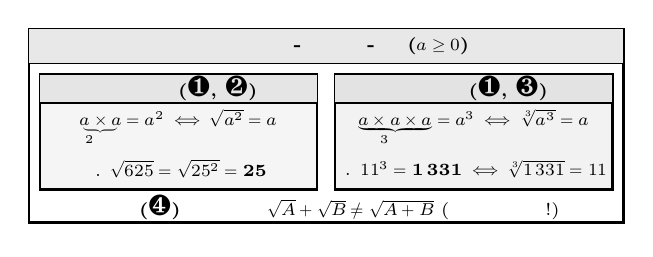
\begin{tikzpicture}[x=1cm, y=1cm, every node/.style={font=\fontsize{6.2pt}{8.1pt}\selectfont, text=black}]
  \draw[black, line width=0.9pt] (0,0) rectangle (7.55,2.46);
  \fill[gray!18] (0,2.02) rectangle (7.55,2.46);
  \draw[black, line width=0.6pt] (0,2.02) -- (7.55,2.02);
  \node at (3.775,2.24) {\textbf{ទំនាក់ទំនងច្រាសរវាងការេ-ឫសការេ និងគូប-ឫសគូប ($a \ge 0$)}};

  % Left: Square <-> Square root
  \draw[black, line width=0.85pt, fill=gray!8] (0.14,0.42) rectangle (3.66,1.88);
  \fill[gray!20] (0.14,1.52) rectangle (3.66,1.88);
  \draw[black, line width=0.5pt] (0.14,1.52) -- (3.66,1.52);
  \node at (1.90,1.70) {\textbf{ការេ និងឫសការេ (\cnum{1}, \cnum{2})}};
  \node at (1.90,1.22) {$\underbrace{a \times a}_{2\text{ កត្តា}} = a^2 \iff \sqrt{a^2} = a$};
  \node at (1.90,0.68) {ឧ. $\sqrt{625} = \sqrt{25^2} = \mathbf{25}$};

  % Right: Cube <-> Cube root
  \draw[black, line width=0.85pt, fill=gray!10] (3.89,0.42) rectangle (7.41,1.88);
  \fill[gray!22] (3.89,1.52) rectangle (7.41,1.88);
  \draw[black, line width=0.5pt] (3.89,1.52) -- (7.41,1.52);
  \node at (5.65,1.70) {\textbf{គូប និងឫសគូប (\cnum{1}, \cnum{3})}};
  \node at (5.65,1.22) {$\underbrace{a\times a\times a}_{3\text{ កត្តា}} = a^3 \iff \sqrt[3]{a^3} = a$};
  \node at (5.65,0.68) {ឧ. $11^3 = \mathbf{1\,331} \iff \sqrt[3]{1\,331} = 11$};

  \node at (3.775,0.19) {\textbf{ប្រយ័ត្ន (\cnum{4})៖} ផលបូករ៉ាឌីកាល់ $\sqrt{A} + \sqrt{B} \ne \sqrt{A + B}$ (ត្រូវបញ្ចេញម្ដងមួយតួ!)};
\end{tikzpicture}}

% ៤. E4 Elaborate: លំហាត់គំរូ និងប្រតិបត្តិទំ.១៣
\newcommand{\figModelsWNOneSeven}{%
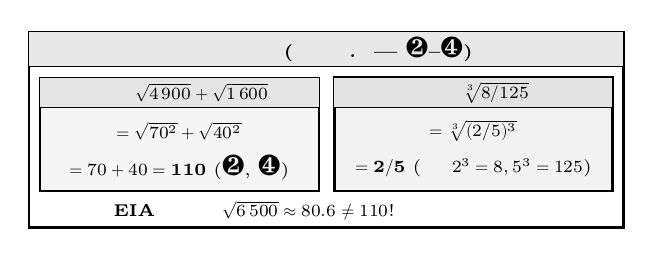
\begin{tikzpicture}[x=1cm, y=1cm, every node/.style={font=\fontsize{6.2pt}{8.2pt}\selectfont, text=black}]
  \draw[black, line width=0.9pt] (0,0) rectangle (7.55,2.48);
  \fill[gray!18] (0,2.04) rectangle (7.55,2.48);
  \draw[black, line width=0.6pt] (0,2.04) -- (7.55,2.04);
  \node at (3.775,2.26) {\textbf{លំហាត់គំរូ ក និង ខ (សៀវភៅគោល ទំ.១៣ — \cnum{2}--\cnum{4})}};

  % Left: Model a
  \draw[black, line width=0.8pt, fill=gray!8] (0.14,0.46) rectangle (3.68,1.90);
  \fill[gray!20] (0.14,1.52) rectangle (3.68,1.90);
  \draw[black, line width=0.5pt] (0.14,1.52) -- (3.68,1.52);
  \node at (1.91,1.71) {\textbf{គំរូ ក៖ $\sqrt{4\,900} + \sqrt{1\,600}$}};
  \node at (1.91,1.22) {$= \sqrt{70^2} + \sqrt{40^2}$};
  \node at (1.91,0.76) {$= 70 + 40 = \mathbf{110}$ (\cnum{2}, \cnum{4})};

  % Right: Model b
  \draw[black, line width=0.85pt, fill=gray!10] (3.88,0.46) rectangle (7.41,1.90);
  \fill[gray!22] (3.88,1.52) rectangle (7.41,1.90);
  \draw[black, line width=0.5pt] (3.88,1.52) -- (7.41,1.52);
  \node at (5.645,1.71) {\textbf{គំរូ ខ៖ $\sqrt[3]{8 / 125}$}};
  \node at (5.645,1.22) {$= \sqrt[3]{(2/5)^3}$};
  \node at (5.645,0.76) {$= \mathbf{2 / 5}$ (ព្រោះ $2^3=8, 5^3=125$)};

  \node at (3.775,0.21) {\textbf{\en{EIA}៖} បើបូកខុសជា $\sqrt{6\,500} \approx 80.6 \ne 110$! ហេតុនេះហាមបូករ៉ាឌីកង់ចូលគ្នា};
\end{tikzpicture}}

% ៥. E5 Evaluate: សំណួរវិនិច្ឆ័យ A-D លើ 4^3 - sqrt(36)
\newcommand{\figExitWNOneSeven}{%
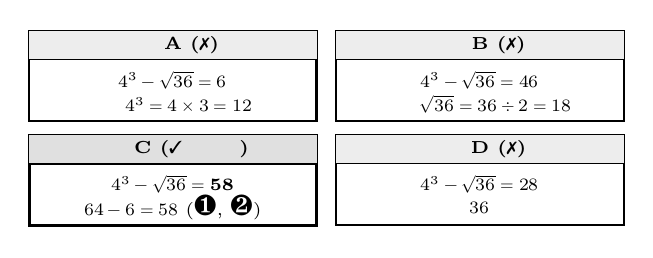
\begin{tikzpicture}[x=1cm, y=1cm, every node/.style={font=\fontsize{6.3pt}{8.2pt}\selectfont, text=black}]
  % Choice A
  \draw[black, line width=0.8pt] (0,1.32) rectangle (3.65,2.46);
  \fill[gray!14] (0,2.10) rectangle (3.65,2.46);
  \draw[black, line width=0.5pt] (0,2.10) -- (3.65,2.10);
  \node at (1.825,2.28) {\textbf{ជម្រើស \en{A} (\ding{55})}};
  \node at (1.825,1.84) {$4^3 - \sqrt{36} = 6$};
  \node at (1.825,1.53) {ច្រឡំ $4^3 = 4\times 3 = 12$};

  % Choice B
  \draw[black, line width=0.8pt] (3.90,1.32) rectangle (7.55,2.46);
  \fill[gray!14] (3.90,2.10) rectangle (7.55,2.46);
  \draw[black, line width=0.5pt] (3.90,2.10) -- (7.55,2.10);
  \node at (5.725,2.28) {\textbf{ជម្រើស \en{B} (\ding{55})}};
  \node at (5.725,1.84) {$4^3 - \sqrt{36} = 46$};
  \node at (5.725,1.53) {ច្រឡំ $\sqrt{36} = 36\div 2 = 18$};

  % Choice C (Correct)
  \draw[black, line width=1.05pt] (0,0) rectangle (3.65,1.14);
  \fill[gray!24] (0,0.78) rectangle (3.65,1.14);
  \draw[black, line width=0.6pt] (0,0.78) -- (3.65,0.78);
  \node at (1.825,0.96) {\textbf{ជម្រើស \en{C} (\ding{51} ត្រឹមត្រូវ)}};
  \node at (1.825,0.52) {$4^3 - \sqrt{36} = \mathbf{58}$};
  \node at (1.825,0.22) {$64 - 6 = 58$ (\cnum{1}, \cnum{2})};

  % Choice D
  \draw[black, line width=0.8pt] (3.90,0) rectangle (7.55,1.14);
  \fill[gray!14] (3.90,0.78) rectangle (7.55,1.14);
  \draw[black, line width=0.5pt] (3.90,0.78) -- (7.55,0.78);
  \node at (5.725,0.96) {\textbf{ជម្រើស \en{D} (\ding{55})}};
  \node at (5.725,0.52) {$4^3 - \sqrt{36} = 28$};
  \node at (5.725,0.22) {ភ្លេចបញ្ចេញ $36$ ពីរ៉ាឌីកាល់};
\end{tikzpicture}}

\begin{document}
\fontsize{10pt}{15.2pt}\selectfont

% ============================================================================
% ក្បាលរដ្ឋបាល (Administrative Header — តាមគំរូ ls_plan.tex)
% ============================================================================
{\centering
  {\muol\fontsize{11pt}{16pt}\selectfont ព្រះរាជាណាចក្រកម្ពុជា\par}
  {\muol\fontsize{11pt}{16pt}\selectfont ជាតិ សាសនា ព្រះមហាក្សត្រ\par}
  \vspace{-3pt}{\khmflourish\par}
}

\vspace{1pt}
{\muol\fontsize{10pt}{15.5pt}\selectfont
មន្ទីរអប់រំ យុវជន និងកីឡា ខេត្តកំពង់ធំ\par
ការិយាល័យអប់រំ យុវជន និងកីឡា ស្រុកកំពង់ស្វាយ\par
អនុវិទ្យាល័យព្រះក្រសាំង\par}

\vspace{2pt}
{\centering{\muol\fontsize{11.5pt}{17pt}\selectfont កិច្ចតែងការបង្រៀន\par}}
\vspace{2pt}

% --- ព័ត៌មានទូទៅ ---
{\hspace*{2.8cm}\renewcommand{\arraystretch}{1.08}
\begin{tabular}{@{}l@{\hspace{0.35cm}}p{2.9cm}@{\hspace{0.15cm}}c@{\hspace{0.25cm}}l@{}}
  - & មុខវិជ្ជា & : & គណិតវិទ្យា ថ្នាក់ទី៧ (ពីជគណិត) \\
  - & ចំណងជើងមេរៀន & : & មេរៀនទី១៖ ចំនួនគត់ \\
  - & ចំណងជើងរង & : & ៨. ការេ គូប និងឫសការេ ឫសគូប (ទំ.១២--១៣) \\
  - & រយៈពេល & : & ១ ម៉ោងសិក្សា (៥០ នាទី) \\
  - & បង្រៀនដោយ & : & ហុក ប៊ុនថែន \\
  - & កាលបរិច្ឆេទ & : & ថ្ងៃពុធ ទី១១ ខែវិច្ឆិកា ឆ្នាំ២០២៦ \\
\end{tabular}\par}

\vspace{2pt}

% --- I. វត្ថុបំណង ---
{\muol\fontsize{10pt}{15.5pt}\selectfont \enbf{I.} វត្ថុបំណង\par}
\vspace{1pt}
{\renewcommand{\arraystretch}{1.10}
\begin{tabular}{@{}p{0.55cm}@{}p{2.35cm}@{\hspace{0.15cm}}c@{\hspace{0.25cm}}p{14.95cm}@{}}
  \hfill\wcirc\hspace{0.2cm} & វិជ្ជាសម្បទា & : & សិស្សប្រាប់បានពីនិយមន័យនៃការេ ($a^2 = a\times a$) គូប ($a^3 = a\times a\times a$) ឫសការេ ($\sqrt{a^2}=a$) និងឫសគូប ($\sqrt[3]{a^3}=a$) ព្រមទាំងស្គាល់ពាក្យបច្ចេកទេស រ៉ាឌីកាល់ និងរ៉ាឌីកង់ បានត្រឹមត្រូវ ។ \\
  \hfill\wcirc\hspace{0.2cm} & បំណិនសម្បទា & : & សិស្សគណនានិងសម្រួលកន្សោមដែលមានការេ គូប ឫសការេ និងឫសគូបនៃចំនួនគត់និងប្រភាគ (ទំ.១២--១៣) លើសន្លឹកកិច្ចការបានត្រឹមត្រូវដោយមិនចាំបាច់ពឹងម៉ាស៊ីនគិតលេខ ។ \\
  \hfill\wcirc\hspace{0.2cm} & ចរិយាសម្បទា & : & សិស្សមានភាពហ្មត់ចត់មិនច្រឡំការលើកជាការេ/គូបជាមួយការគុណនឹង $2$ ឬ $3$ មានទម្លាប់ផ្ទៀងផ្ទាត់ច្រាសទៅមក និងសហការដោះស្រាយលំហាត់ជាក្រុម ។ \\
\end{tabular}\par}

\vspace{2pt}

% --- II. សម្ភារៈឧបទេស ---
{\muol\fontsize{10pt}{15.5pt}\selectfont \enbf{II.} សម្ភារៈឧបទេស\par}
\vspace{1pt}
\hspace*{0.55cm}$\bullet$\ សៀវភៅសិក្សាគោលថ្នាក់ទី៧ (ទំ.១២--១៤) ក្ដារខៀន ដីស/ហ្វឺត បន្ទាត់ត្រង់ និង\textbf{សន្លឹកកិច្ចការសិស្សបំពេញចន្លោះ ស-ខ្មៅ} (កូដ \en{WN17} ទំព័រ ១--២ សម្រាប់សិស្ស និងទំព័រ ៣ ប្លង់ក្ដារខៀន/ចម្លើយគ្រូ — គ្មានប្រើ \en{LCD})\par

\vspace{2pt}

% --- III. វិធីសាស្រ្តបង្រៀន ---
{\muol\fontsize{10pt}{15.5pt}\selectfont \enbf{III.} វិធីសាស្រ្តបង្រៀន\par}
\vspace{1pt}
{\renewcommand{\arraystretch}{1.08}
\begin{tabular}{@{}p{0.55cm}@{}p{2.35cm}@{\hspace{0.15cm}}c@{\hspace{0.25cm}}p{14.95cm}@{}}
  \hfill$\bullet$\hspace{0.2cm} & គោលវិធី & : & សិស្សមជ្ឈមណ្ឌល (សន្លឹកកិច្ចការបំពេញចន្លោះជាគោល + ការពិភាក្សាជាក្រុមតូច ៣ នាក់) \\
  \hfill$\bullet$\hspace{0.2cm} & យុទ្ធវិធីបង្រៀន & : & គំរូស្ថាបនានិយម \en{5Es} រួមបញ្ចូល \textbf{គំរូធរណីមាត្រការេ-គូប (\en{Geometric Area/Volume Representation})} និង \textbf{ការបំប្លែងច្រាសរ៉ាឌីកាល់ (\en{Inverse Radical Mapping})} \\
\end{tabular}\par}

\vspace{2pt}

% --- IV. ដំណើរការបង្រៀន ---
{\muol\fontsize{10pt}{15.5pt}\selectfont \enbf{IV.} ដំណើរការបង្រៀន\par}

{\renewcommand{\arraystretch}{1.15}
\begin{longtable}{|L{5.50cm}|L{7.90cm}|L{4.80cm}|}
\hline
\multicolumn{1}{|c|}{\cellcolor{headgray}\muol សកម្មភាពគ្រូ} &
\multicolumn{1}{c|}{\cellcolor{headgray}\muol ខ្លឹមសារមេរៀន} &
\multicolumn{1}{c|}{\cellcolor{headgray}\muol សកម្មភាពសិស្ស} \\
\hline
\endfirsthead

\hline
\multicolumn{1}{|c|}{\cellcolor{headgray}\muol សកម្មភាពគ្រូ} &
\multicolumn{1}{c|}{\cellcolor{headgray}\muol ខ្លឹមសារមេរៀន} &
\multicolumn{1}{c|}{\cellcolor{headgray}\muol សកម្មភាពសិស្ស} \\
\hline
\endhead

% ==================== ជំហានទី១ (2min) ====================
\stepheader{ជំហានទី១ \enbf{(}រដ្ឋបាលថ្នាក់\enbf{)}}
$\bullet$ ពិនិត្យវត្តមាន អនាម័យ និងសណ្ដាប់ធ្នាប់ថ្នាក់រៀន \par
$\bullet$ រៀបចំក្រុមតូច ៣ នាក់តាមតុ និងចែក\textbf{សន្លឹកកិច្ចការសិស្ស (\en{WN17} ទំព័រ ១–២)}
&
$\bullet$ រដ្ឋបាលថ្នាក់ អនាម័យ និងវិន័យសិក្សា \par
$\bullet$ ចែកសន្លឹកកិច្ចការម្នាក់ ១ សន្លឹក សម្រាប់បំពេញតាមដំណាក់កាល \en{E1--E5}
&
$\circ$ ប្រធានថ្នាក់រាយការណ៍វត្តមានសិស្ស \par
$\circ$ ទទួលសន្លឹកកិច្ចការ សរសេរឈ្មោះ និងអង្គុយតាមក្រុម ៣ នាក់ \\
\hline

% ==================== ជំហានទី២ (9min: កំណែ <=3m + រំលឹក 3m + E1 3m) ====================
\stepheader{ជំហានទី២ \enbf{(}កិច្ចការផ្ទះ \enbf{+} ទំនាក់ទំនងមេរៀនថ្មី\enbf{)}}
\ditem \textbf{កំណែកិច្ចការផ្ទះ ($\le\text{\enbf{3\,min}}$)} \par
$\bullet$ ហៅសិស្សផ្ទៀងផ្ទាត់ចម្លើយលំហាត់ទំ.១៤ លេខ ៦ និង លេខ ៧ លើក្ដារខៀនផ្នែកឆ្វេង
&
{\centering\redsub{កំណែកិច្ចការផ្ទះមេរៀនមុន (ទំ.១៤ លេខ ៦ និង លេខ ៧)}\par}
$\bullet$ \textbf{លេខ ៦ ក (ដប់; រយ; ពាន់)៖} $149\,910;\ 149\,900;\ 150\,000$ (\emph{ខ, គ, ឃ ផ្ទៀងលើក្ដារខៀន}) \par
$\bullet$ \textbf{លេខ ៧៖} ក. $\approx \mathbf{900}$ \quad ខ. $\approx \mathbf{3\,600\,000}$ \quad គ. $4\,200\div 60 = \mathbf{70}$
&
$\circ$ ផ្ទៀងចម្លើយលេខ ៦ និង លេខ ៧ រួចកែចូលសៀវភៅ \\[3pt]

\ditem \textbf{រំលឹកមេរៀនទាក់ទង (\enbf{3min})} \par
$\bullet$ គូររូបការេជ្រុង $a$ និងគូបទ្រនុង $a$ លើក្ដារខៀន រួចសួររូបមន្តផ្ទៃក្រឡាការេ និងមាឌគូប
&
{\centering\redsub{រំលឹករូបមន្តផ្ទៃក្រឡាការេ និងមាឌគូប}\par}
$\bullet$ ផ្ទៃក្រឡាការេជ្រុង $a$៖ $S = a \times a$ \par
$\bullet$ មាឌគូបទ្រនុង $a$៖ $V = a \times a \times a$
&
$\circ$ ឆ្លើយ៖ «$S = a \times a$ និង $V = a \times a \times a$!» \\[3pt]

$\bullet$ សួរបន្ត៖ «ចុះបើដឹងផ្ទៃការេស្មើ $36\unit{cm}^2$ តើជ្រុងរបស់វាមានប្រវែងប៉ុន្មានសង់ទីម៉ែត្រ?»
&
$\bullet$ ដោយ $6 \times 6 = 36$ នោះជ្រុងការេមានប្រវែងស្មើនឹង $6\unit{cm}$
&
$\circ$ ឆ្លើយ៖ «ស្មើនឹង $6\unit{cm}$ ព្រោះ $6 \times 6 = 36$!» \\[3pt]

\fiveE{E1 - Engage (3min)} \timenote{(កុំទាន់ផ្ដល់ចម្លើយ)} \par
\ditem \textbf{បេសកកម្មអន្ទាក់ស្វ័យគុណ $5^2$ និង $5^3$ (សន្លឹកកិច្ចការ \en{E1})} \par
$\bullet$ ឱ្យសិស្សពិនិត្យប្រអប់ \en{E1} លើការគណនា $5^2$ និង $5^3$ (ឧទាហរណ៍ ៨.១ ទំ.១២) រវាង\textbf{សិស្ស ក} និង\textbf{សិស្ស ខ}
&
\redsub{បេសកកម្ម \en{E1}៖ រកផ្ទៃការេជ្រុង $5\unit{cm}$ ($5^2$) និងមាឌគូបទ្រនុង $5\unit{cm}$ ($5^3$)} \par
$\bullet$ \textbf{សិស្ស ក} សរសេរ $5^2 = 10\unit{cm}^2$ និង $5^3 = 15\unit{cm}^3$ \par
$\bullet$ \textbf{សិស្ស ខ} សរសេរ $5^2 = 25\unit{cm}^2$ និង $5^3 = 125\unit{cm}^3$ ។ តើអ្នកណាត្រឹមត្រូវ?
&
$\circ$ ពិភាក្សាជាគូ និងគូស \ding{51} ក្នុងប្រអប់ \en{E1} លើសន្លឹកកិច្ចការ \\[3pt]

&
\cfig{\figEngageWNOneSeven}
& \\
\hline

% ==================== ជំហានទី៣ (17min: E2 11m + E3 6m) ====================
\stepheader{ជំហានទី៣ \enbf{(}ខ្លឹមសារមេរៀនថ្មី\enbf{)}}
\fiveE{E2 - Explore (11min)} \par
$\bullet$ សរសេរចំណងជើងរង \textbf{៨. ការេ គូប និងឫសការេ ឫសគូប} លើក្ដារខៀន \par
\ditem \textbf{សកម្មភាព ១៖ ៨.១ ការេនិងគូប (សៀវភៅគោល ទំ.១២, \enbf{5min}, \en{E2-A})} \par
$\bullet$ ឱ្យសិស្សបំពេញការគណនាផ្ទៃក្រឡាការេជ្រុង $5\unit{cm}$ និងមាឌគូបទ្រនុង $5\unit{cm}$ លើ \en{E2-A}
&
៨. ការេ គូប និងឫសការេ ឫសគូប \par
$\bullet$ \textbf{៨.១ ការេនិងគូប (ទំ.១២)៖} ផ្ទៃក្រឡាការេ $\underbrace{5 \times 5}_{2\text{ កត្តា}} = 5^2 = \mathbf{25}\unit{cm}^2$ (\emph{ប្រាំការេ}) \par
\hspace*{0.2cm}មាឌគូប $\underbrace{5 \times 5 \times 5}_{3\text{ កត្តា}} = 5^3 = \mathbf{125}\unit{cm}^3$ (\emph{ប្រាំគូប})
&
$\circ$ រាប់ចំនួនកត្តាដូចគ្នា ឃើញ $5^2 = 25$ និង $5^3 = 125$ \\[3pt]

\ditem \textbf{សកម្មភាព ២៖ ៨.២ ឫសការេនិងឫសគូប និងសម្គាល់ (ទំ.១២--១៣, \enbf{6min}, \en{E2-B})} \par
$\bullet$ ឱ្យសិស្សរកជ្រុងការេពីផ្ទៃ $S = 100\unit{cm}^2$ និងទ្រនុងគូបពីមាឌ $V = 27\unit{dm}^3$ លើ \en{E2-B}
&
$\bullet$ \textbf{៨.២ ឫសការេនិងឫសគូប (ទំ.១២)៖} \par
\hspace*{0.2cm}១) $S = 100\unit{cm}^2 = 10\unit{cm}\times 10\unit{cm} \implies a = \sqrt{100} = \sqrt{10^2} = \mathbf{10}\unit{cm}$ \par
\hspace*{0.2cm}២) $V = 27\unit{dm}^3 = 3\unit{dm}\times 3\unit{dm}\times 3\unit{dm} \implies a = \sqrt[3]{27} = \sqrt[3]{3^3} = \mathbf{3}\unit{dm}$
&
$\circ$ បំពេញប្រវែងជ្រុងការេ $10\unit{cm}$ និងទ្រនុងគូប $3\unit{dm}$ \\[3pt]

$\bullet$ ណែនាំពាក្យ \textbf{រ៉ាឌីកាល់} និង\textbf{រ៉ាឌីកង់} ព្រមទាំងឧទាហរណ៍ ៨.៣ (ទំ.១៣៖ $\sqrt{625}, \ 9^2, \ 11^3$)
&
$\bullet$ \textbf{សម្គាល់ និង ៨.៣ (ទំ.១៣)៖} សញ្ញា $\sqrt{\ }, \sqrt[3]{\ }$ ហៅថា\textbf{រ៉ាឌីកាល់}; $100, 27$ ហៅថា\textbf{រ៉ាឌីកង់} \par
\hspace*{0.2cm}គណនាដោយបំបែកកត្តា ឬផ្ទៀងគ្រាប់ចុចទំ.១៣៖ $\sqrt{625}=\mathbf{25}, \ 9^2=\mathbf{81}, \ 11^3=\mathbf{1\,331}$
&
$\circ$ កត់ត្រាពាក្យរ៉ាឌីកាល់/រ៉ាឌីកង់ និងគណនា $25, 81, 1\,331$ \\[3pt]

&
\cfig{\figGeomWNOneSeven}
& \\[3pt]

% --- E3 Explain (6min) ---
\fiveE{E3 - Explain (6min)} \par
$\bullet$ ដឹកនាំសិស្សសង្ខេបរូបមន្តច្រាសរវាងស្វ័យគុណ និងរ៉ាឌីកាល់ ($a \ge 0$) លើ \en{E3}
&
$\bullet$ \textbf{សង្ខេបនិយមន័យ និងរូបមន្តច្រាស ($a \ge 0$)៖} \par
\hspace*{0.15cm}១) ការេ និងឫសការេ៖ \graybox{$a^2 = a \times a$} $\iff$ \graybox{$\sqrt{a^2} = a$} \par
\hspace*{0.15cm}២) គូប និងឫសគូប៖ \graybox{$a^3 = a \times a \times a$} $\iff$ \graybox{$\sqrt[3]{a^3} = a$}
&
$\circ$ បំពេញប្រអប់រូបមន្តច្រាសទាំងពីរលើ \en{E3} \\[3pt]

$\bullet$ ភ្ជាប់\textbf{ធនាគារហេតុផល \cnum{1}} លើក្ដារខៀន និងសន្លឹកកិច្ចការ
&
\textbf{ធនាគារហេតុផល (\en{Warrant Bank})៖} \par
\cnum{1} \textbf{និយមន័យការេ/គូប៖} $a^2 = a\times a$ ($\ne 2a$); $a^3 = a\times a\times a$ ($\ne 3a$)
&
$\circ$ ផ្ទៀងលេខកូដ \cnum{1} លើសន្លឹកកិច្ចការ \\[3pt]

$\bullet$ ភ្ជាប់\textbf{ធនាគារហេតុផល \cnum{2}} សម្រាប់និយមន័យឫសការេ ($a \ge 0$)
&
\cnum{2} \textbf{ឫសការេ ($a\ge 0$)៖} $\sqrt{a^2} = a$ (រកចំនួនមិនអវិជ្ជមានដែលការេស្មើរ៉ាឌីកង់)
&
$\circ$ ផ្ទៀងលេខកូដ \cnum{2} លើសន្លឹកកិច្ចការ \\[3pt]

$\bullet$ ភ្ជាប់\textbf{ធនាគារហេតុផល \cnum{3}--\cnum{4}} សម្រាប់ឫសគូប និងការគណនាកន្សោមរ៉ាឌីកាល់
&
\cnum{3} \textbf{ឫសគូប៖} $\sqrt[3]{a^3} = a$ និងចំពោះប្រភាគ $\sqrt[3]{a^3 / b^3} = a / b$ ($b\ne 0$) \par
\cnum{4} \textbf{ប្រយ័ត្នផលបូករ៉ាឌីកាល់៖} ត្រូវបញ្ចេញពីរ៉ាឌីកាល់ម្ដងមួយតួ ($\sqrt{A}+\sqrt{B} \ne \sqrt{A+B}$)
&
$\circ$ ផ្ទៀងលេខកូដ \cnum{3}--\cnum{4} លើសន្លឹកកិច្ចការ \\[3pt]

&
\cfig{\figInverseRadWNOneSeven}
& \\
\hline

% ==================== ជំហានទី៤ (20min: E4 10m + E5 10m) ====================
\stepheader{ជំហានទី៤ \enbf{(}ពង្រីកចំណេះដឹង\enbf{)}}
\fiveE{E4 - Elaborate (10min)} \par
\ditem \textbf{លំហាត់គំរូ ក និង ខ៖ កន្សោមឫសការេ និងឫសគូបប្រភាគ (ទំ.១៣)} \par
$\bullet$ ឱ្យសិស្សដោះស្រាយលំហាត់គំរូ ក ($\sqrt{4\,900} + \sqrt{1\,600}$) លើសន្លឹកកិច្ចការ \en{E4}
&
{\muol លំហាត់គំរូ} \textbf{(សៀវភៅគោល ទំ.១៣)៖} \par
$\bullet$ \textbf{ក.} $\sqrt{4\,900} + \sqrt{1\,600} = \sqrt{70^2} + \sqrt{40^2} = 70 + 40 = \graybox{$110$}$ (\cnum{2}, \cnum{4})
&
$\circ$ បំបែក $4\,900 = 70^2$ និង $1\,600 = 40^2$ បូកឃើញ $110$ \\[3pt]

$\bullet$ ឱ្យសិស្សដោះស្រាយលំហាត់គំរូ ខ ($\sqrt[3]{\frac{8}{125}}$) លើសន្លឹកកិច្ចការ \en{E4}
&
$\bullet$ \textbf{ខ.} $\sqrt[3]{\dfrac{8}{125}} = \sqrt[3]{\dfrac{2}{5}\times\dfrac{2}{5}\times\dfrac{2}{5}} = \sqrt[3]{\left(\dfrac{2}{5}\right)^3} = \graybox{$\dfrac{2}{5}$}$ (\cnum{3})
&
$\circ$ សរសេរ $\frac{8}{125} = \left(\frac{2}{5}\right)^3$ បញ្ចេញពីឫសគូបឃើញ $\frac{2}{5}$ \\[3pt]

&
\cfig{\figModelsWNOneSeven}
& \\[3pt]

$\bullet$ សួរសំណួរឆ្លុះបញ្ចាំង \textbf{\en{EIA Looking-Back} (1min)} បំបែកអន្ទាក់បូករ៉ាឌីកង់
&
\textbf{\en{EIA Looking-Back}៖} «បើសិស្សម្នាក់បូកខុសជា $\sqrt{4\,900 + 1\,600} = \sqrt{6\,500}$ តើស្មើ $110$ ដែរឬទេ?» ($\to$ ទេ! ព្រោះ $110^2 = 12\,100 \ne 6\,500$ រីឯ $80^2 = 6\,400$!)
&
$\circ$ ផ្ទៀងផ្ទាត់ឃើញថា $\sqrt{A}+\sqrt{B}$ មិនស្មើ $\sqrt{A+B}$ ឡើយ \\[3pt]

% --- E5 Evaluate (10min) ---
\fiveE{E5 - Evaluate (10min)} \par
\ditem \textbf{ប្រតិបត្តិជាក្រុមតូច ៣ នាក់ (4min, សន្លឹកកិច្ចការ \en{E5})} \par
$\bullet$ ឱ្យក្រុមសិស្សដោះស្រាយលំហាត់ប្រតិបត្តិទំ.១៣ ($\sqrt{12^2}\times\sqrt{34^2}$ និង $\sqrt[3]{\frac{216}{1\,000}}$)
&
{\muol លំហាត់ប្រតិបត្តិ} \textbf{(សៀវភៅគោល ទំ.១៣)៖} \par
$\bullet$ \textbf{១)} $\sqrt{12^2} \times \sqrt{34^2} = 12 \times 34 = \graybox{$408$}$ (\cnum{2}) \par
$\bullet$ \textbf{២)} $\sqrt[3]{\dfrac{216}{1\,000}} = \sqrt[3]{\left(\dfrac{6}{10}\right)^3} = \dfrac{6}{10} = \graybox{$\dfrac{3}{5}$}$ (\cnum{3})
&
$\circ$ សហការគ្នាគណនាឃើញ $408$ និងសម្រួលប្រភាគឃើញ $\frac{3}{5}$ \\[3pt]

$\bullet$ ឱ្យក្រុមសិស្សផ្ទៀងផ្ទាត់និង\textbf{បិទបេសកកម្ម \en{E1} (2min)}
&
$\bullet$ \textbf{បិទបេសកកម្ម \en{E1}៖} \textbf{សិស្ស ខ} ត្រឹមត្រូវ! $5^2 = 5\times 5 = \mathbf{25}\unit{cm}^2$ និង $5^3 = 5\times 5\times 5 = \mathbf{125}\unit{cm}^3$ (\cnum{1}) ។
&
$\circ$ បិទបេសកកម្ម \en{E1} ឃើញសិស្ស ខ ត្រឹមត្រូវ ($25$ និង $125$) \\[3pt]

\ditem \textbf{សំណួរវិនិច្ឆ័យ \en{A--D} និងសំបុត្រចេញ (4min)} \par
$\bullet$ សរសេរកន្សោម $4^3 - \sqrt{36}$ និងជម្រើស \en{A--D} លើក្ដារខៀន
&
{\centering\textbf{សំណួរវិនិច្ឆ័យ \en{A--D}៖ តើតម្លៃនៃកន្សោម $4^3 - \sqrt{36}$ ស្មើនឹងប៉ុន្មាន?}\par}
&
$\circ$ គណនា $4^3 = 64$ និង $\sqrt{36} = 6$ រួចដក $64 - 6 = 58$ \\[3pt]

$\bullet$ ឱ្យសិស្សគូសរង្វង់ជម្រើសត្រូវលើសន្លឹកកិច្ចការ រួចលើកម្រាមដៃ ១--៤ ព្រមគ្នា
&
$\bullet$ វិភាគកំហុសក្នុងជម្រើស \en{A} ($6$), \en{B} ($46$), \en{D} ($28$) តាមលេខកូដហេតុផល \cnum{1} និង \cnum{2}
&
$\circ$ គូសរង្វង់លើសន្លឹកកិច្ចការ និងលើកម្រាមដៃ ៣ (\textbf{ជម្រើស \en{C}}) \\[3pt]

&
\cfig{\figExitWNOneSeven}
& \\[3pt]

$\bullet$ បញ្ជាក់ចម្លើយត្រូវ (\textbf{ជម្រើស \en{C}}) និងឱ្យបំពេញ\textbf{សំបុត្រចេញ ៦០ វិនាទី}
&
$\bullet$ \textbf{សំបុត្រចេញ៖} គណនា $3^3 + \sqrt[3]{64} = 27 + 4 = \mathbf{31}$ (\cnum{1}, \cnum{3}) ។
&
$\circ$ បំពេញសំបុត្រចេញឃើញ $31$ មុនបញ្ចប់ម៉ោង \\
\hline

% ==================== ជំហានទី៥ (<=2min) ====================
\stepheader{ជំហានទី៥ \enbf{(}កិច្ចការផ្ទះ \enbf{+} បណ្ដាំផ្ញើ\enbf{)}}
\timenote{ចំណាយពេលឱ្យតិចបំផុតកុំឱ្យលើស 2min} \par
$\bullet$ ណែនាំប្រអប់\textbf{កិច្ចការផ្ទះបញ្ចប់មេរៀនទី១}លើសន្លឹកកិច្ចការទំព័រ ២ (ទំ.១៤ លេខ ៨ និង លេខ ៩)
&
{\centering{\muol កិច្ចការផ្ទះ} \textbf{(សៀវភៅគោល ទំ.១៤ លេខ ៨ និង លេខ ៩)}\par} \par
$\bullet$ \textbf{លេខ ៨៖} ក. $2^2 \times 5^3$ \quad ខ. $5^3 + 3^2$ \quad គ. $8^2 - 3^3$ \quad ឃ. $3x^2$ បើ $x = 5$ \par
$\bullet$ \textbf{លេខ ៩៖} ក. $\sqrt{9}\times\sqrt{16}$ \quad ខ. $4^2 - \sqrt{4}$ \quad គ. $\sqrt{100}\times\sqrt{196}$ \quad ឃ. $\dfrac{5^3 + \sqrt[3]{64} - \sqrt[3]{8}}{3^3}$
&
$\circ$ គូសចំណាំលំហាត់ទំ.១៤ លេខ ៨ និង លេខ ៩ \\[3pt]

$\bullet$ ផ្ដាំផ្ញើឱ្យរំលឹកសង្ខេបមេរៀនទី១ ទាំងមូល និងអានមុនមេរៀនទី២ (ទំ.១៥–១៧)
&
$\bullet$ \textbf{បណ្ដាំផ្ញើ៖} បញ្ចប់លំហាត់មេរៀនទី១ ទាំងអស់ និងអានមុន \textbf{មេរៀនទី២៖ តួចែកនិងពហុគុណ} (ទំ.១៥–១៧) ។
&
$\circ$ កត់ត្រាបណ្ដាំផ្ញើ ទុកសន្លឹកកិច្ចការក្នុងសៀវភៅ និងជម្រាបលាគ្រូ \\
\hline
\end{longtable}}

\vspace{6pt}
% --- ហត្ថលេខា (កាលបរិច្ឆេទត្រូវគ្នា ១០០% នឹងខាងលើ) ---
{\centering
\hspace*{5.2cm}\begin{minipage}{11.5cm}
  \centering
  ថ្ងៃពុធ ២កើត ខែកត្តិក ឆ្នាំមមី អដ្ឋស័ក ពុទ្ធសករាជ ២៥៧០\par
  កំពង់ស្វាយ, ថ្ងៃទី១១ ខែវិច្ឆិកា ឆ្នាំ២០២៦\par
  \vspace{2pt}
  {\muol គ្រូបង្រៀន\par}
  \vspace{32pt}
  \hfill{\muol ហុក ប៊ុនថែន}\hspace*{1.4cm}
\end{minipage}\par}

\end{document}
